
\section{Physical prototype description}
In this section, we will describe everything about the hardware side of this project.

\subsection{Software package}

The following different pieces of software were used to create this prototype:

\begin{itemize}
    \item Raspbian OS 32-bit\cite{raspbian}: Linux distribution used in the Raspberry Pi.
    \item Fritzing\cite{fritzing}: Software package used to generate the connection graphics for the electronics components.
    \item Autodesk Fusion 360\cite{fusion360}: CAD program used to design printable parts needed for the robot.
\end{itemize}


    

\subsection{Hardware used}

The following list contains all the hardware we used for our robot:

\begin{itemize}
    \item \textbf{SG-90 servomotors}: chosen for their size and respectable 1.3 Kg-cm torque. 
    \item \textbf{Raspberry Pi 4B 8GB}: chosen as the main controller for the robot. The extra RAM memory is needed as the internal GPU shares memory with the CPU.
    
    \item \textbf{PCA9685 12-Channel PWM Driver}: The Raspberry Pi only has a few hardware PWM enabled pins, with only two PWM channels available. Several software-based solutions use more pins as PWM-enabled pins with more channels, but we found these to negatively affect the robot's performance, and in any case, powering the servos becomes cumbersome. As a result, we used an I2C based PWM generator, the PCA9685 12-Channel PWM Driver. This component can be connected to the Raspberry Pi through the I2C interface, does not rely on the Pi's CPU to accurately generate the pulses needed to drive our three motors, and has the added benefit of having its power lines for the motors.
    \item \textbf{3.3v 1S LiPo Battery + Adafruit Powerboost 1000C}: Step-up voltage regulator with undervoltage protection for our LiPo battery. This will be used to power the servomotors.
    
    \item \textbf{Qualcomm Quickcharge 3.0/USB Power delivery capable USB battery}: This battery will be used to power the Raspberry Pi. Either QC3.0 or USB PD is needed to provide 3A at 5V of power to the Raspberry Pi.
    
    \item \textbf{7 Inch HDMI Display}: This display allows us to show users a live style transfer of the camera feed.
    \end{itemize}

    \begin{figure}[h]
        \centering
        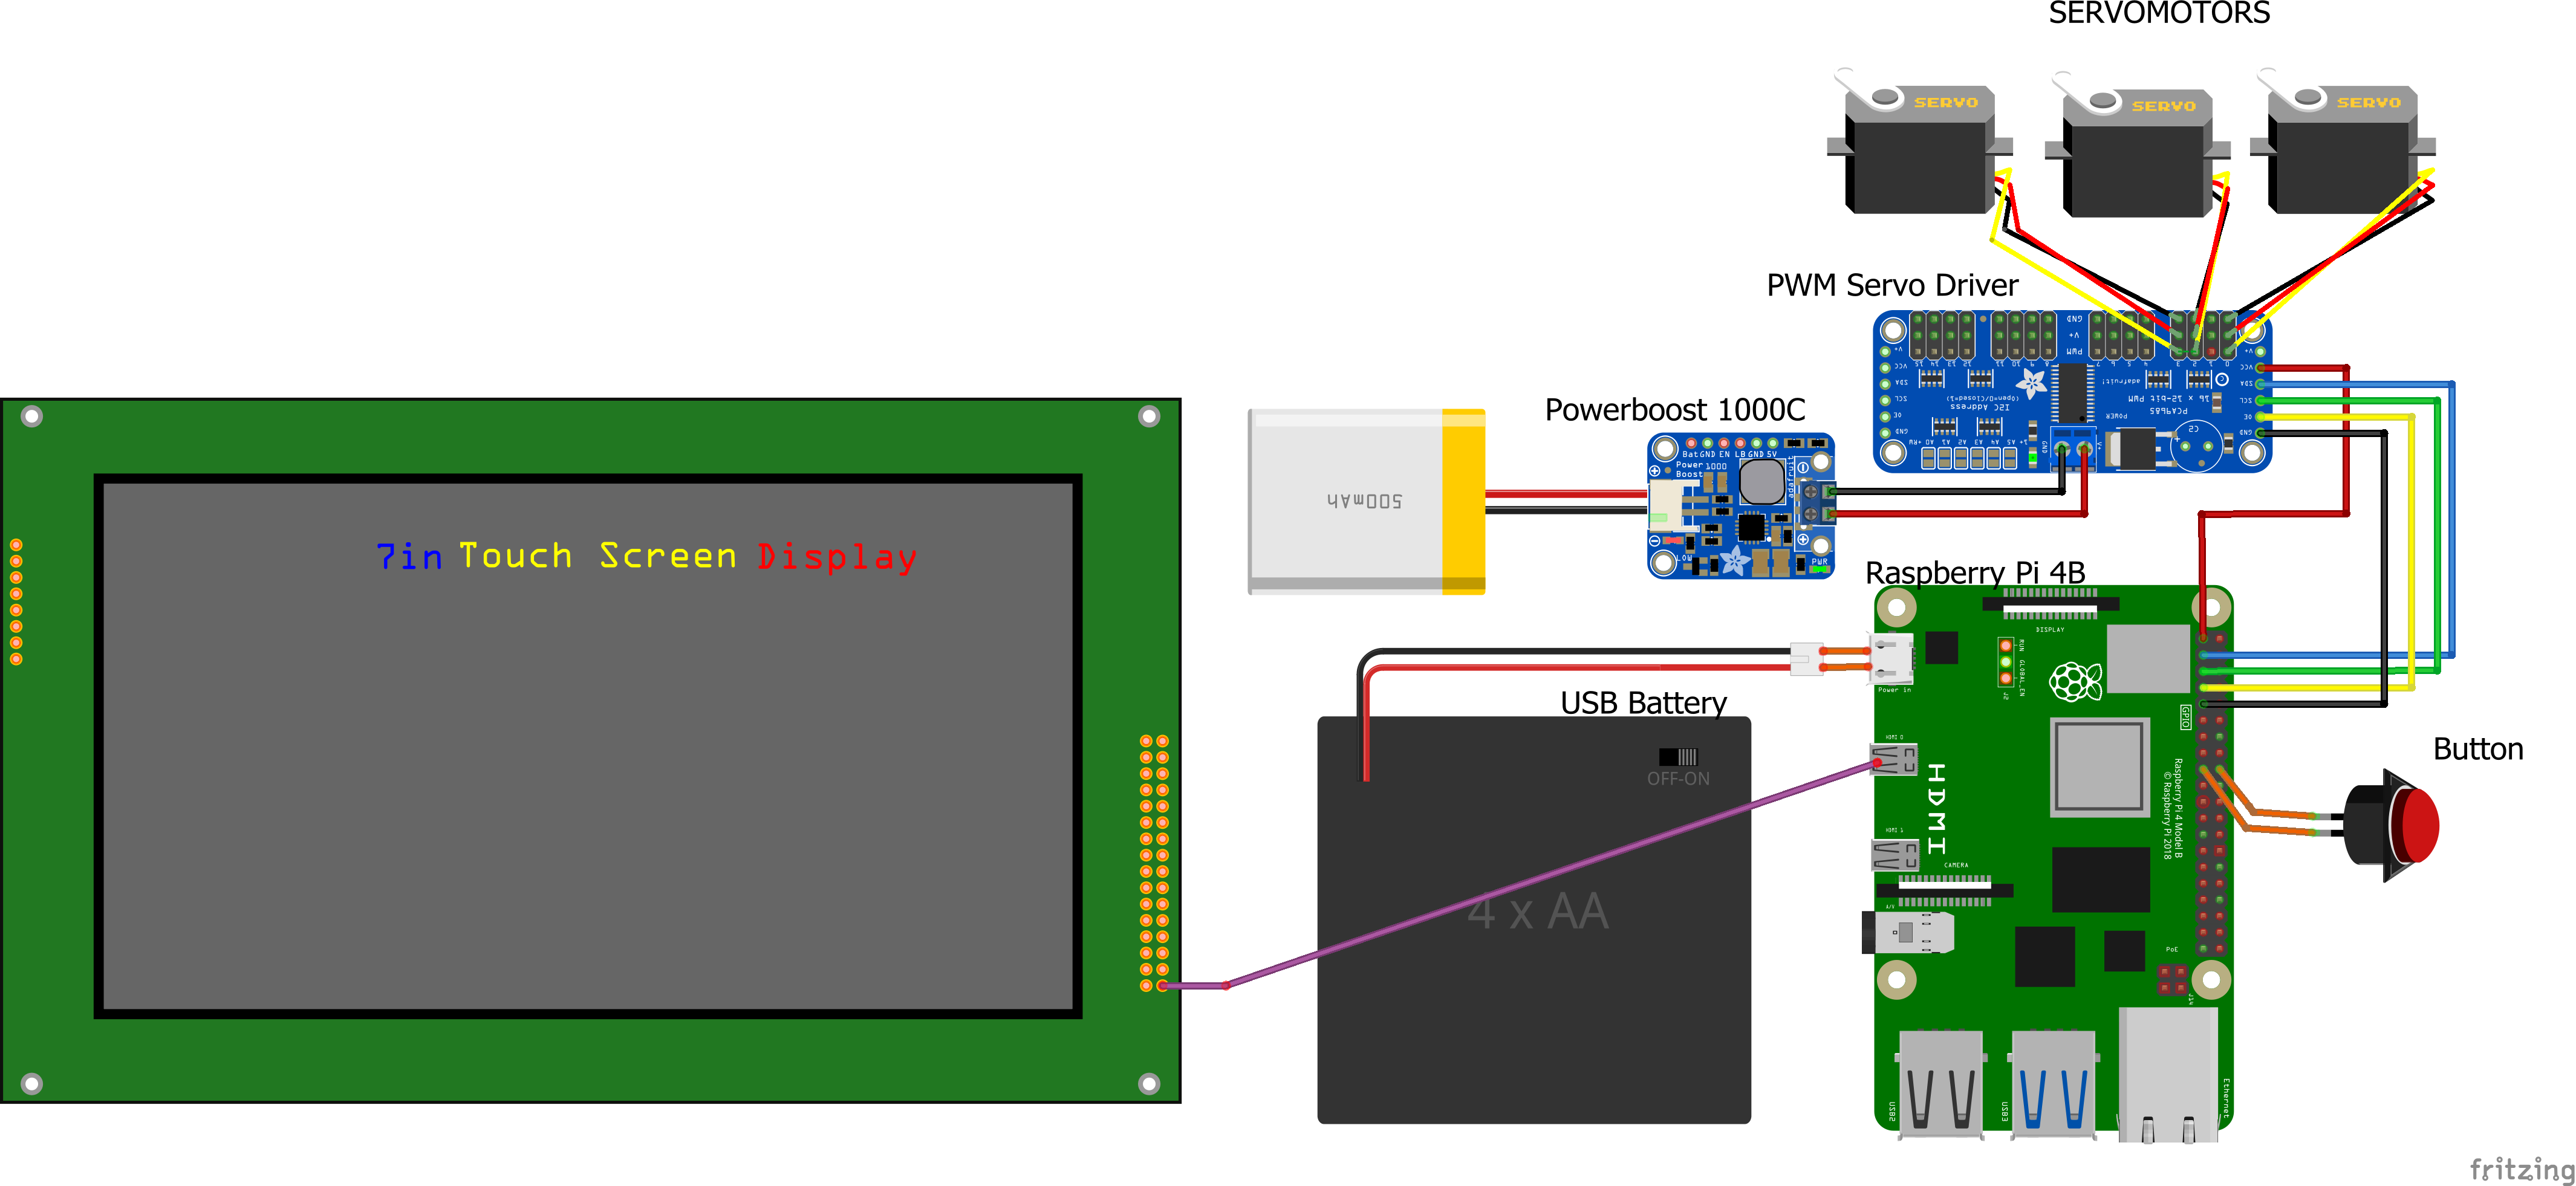
\includegraphics[width =0.7\textwidth]{resources/fritzing.png}
        \caption{Connection diagram of the final hardware configuration.}\label{fig:hardware_configuration}
    \end{figure}  
    



\subsection{3D printed parts}

We redesigned the previous robot completely, as some of the STL files used to print the parts had errors. We took advantage of the occasion to bake in some extra features like consideration for a small USB battery and lipo battery to stop relying on outlets, places to route the cables internally, a button to interact with the robot, and a redesigned that allows for a small fan to be placed above the Raspberry Pi 4B's CPU heatsink. 


\begin{figure}[h]
    \centering
    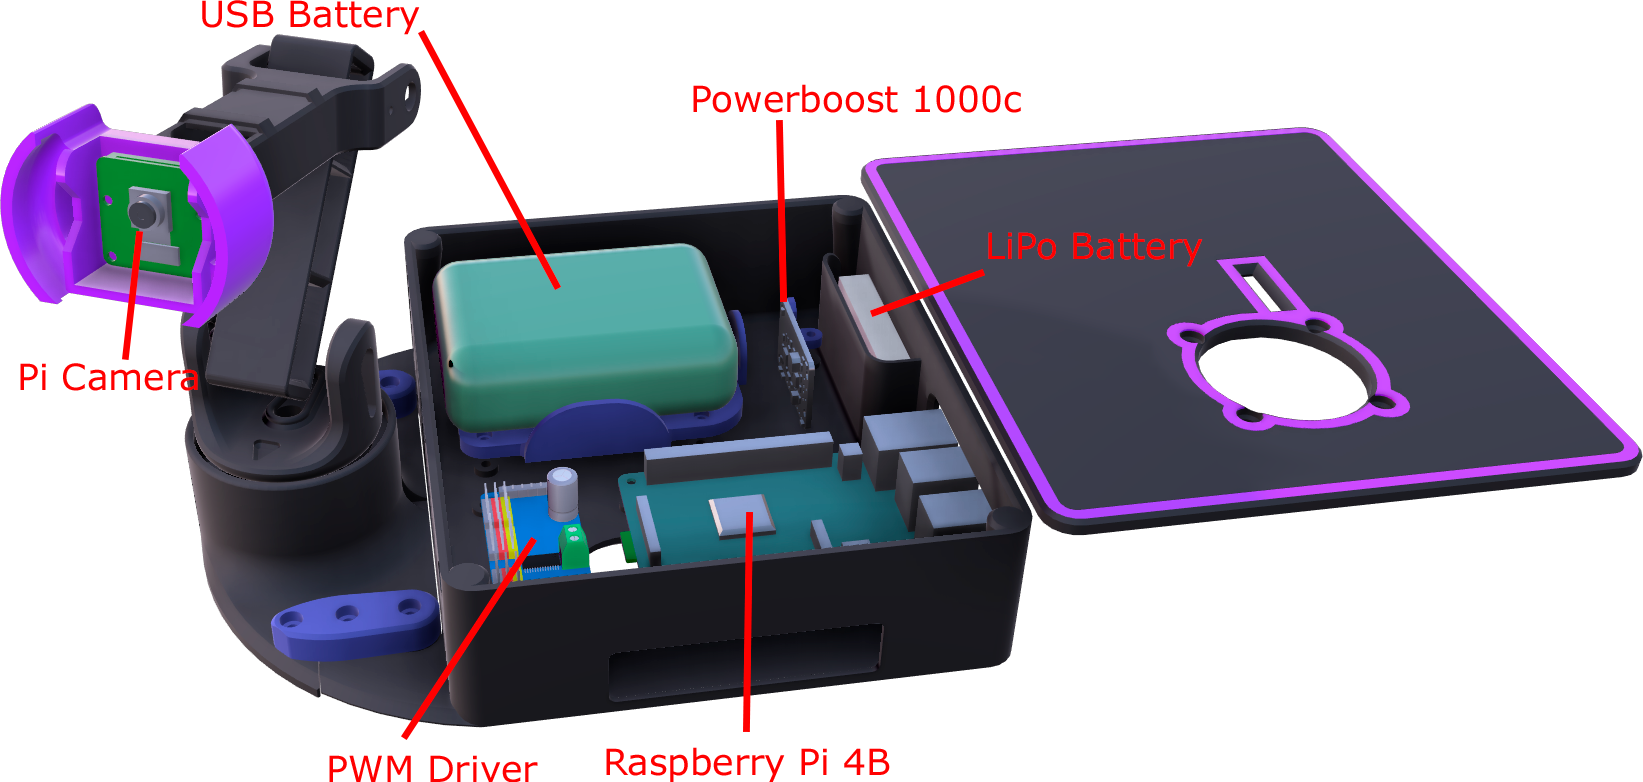
\includegraphics[width = 0.8\textwidth]{resources/final_robot_assembly_view2.png}
    \caption{3D model with components.}\label{fig:robot_assembly_view_2}
\end{figure}


In Figure \ref{fig:robot_assembly_view_2} you can see the final render of the 3D model with mockups of the hardware and the labels for the components inside of the robot. 
